\chapter{Introducción y objetivos}

\section{Introducción}
La Formula Student es una competición internacional que desafía a estudiantes de ingeniería de todo el mundo a diseñar, construir y competir con monoplazas diseñados, construidos y pilotados por los mismos estudiantes. Esta competición proporciona una plataforma excepcional para que los futuros ingenieros pongan en práctica sus conocimientos y adquieran experiencia práctica en todos los ámbitos de la ingeniería, desde la manufactura hasta la gestión de proyectos. El énfasis en la innovación, la eficiencia y la adaptabilidad aporta un valor incalculable a la formación de los jóvenes ingenieros.

Dentro de los puntos clave de la Formula Student en los últimos años, se encuentra el interés creciente en la tracción eléctrica. En un mundo cada vez más preocupado por la sostenibilidad y la eficiencia energética, los motores eléctricos han surgido como una opción atractiva para la propulsión de vehículos de potencias y autonomías cada vez más elevadas. Este cambio de paradigma plantea la cuestión fundamental de cómo diseñar y controlar eficazmente los sistemas eléctricos para lograr un alto rendimiento sin dejar de ser accesibles para el público general. La optimización de costes no suele ser un reto en los deportes de motor, incluida la Formula Student, pero la innovación que se lleva a cabo en estos contextos de libertad absoluta permite traer ideas de las competiciones a los vehículos de calle. En este contexto, se establece un puente fundamental entre el presente y el futuro de la movilidad sostenible, explorando los elementos técnicos que impulsan el rendimiento de los motores eléctricos y su control, contribuyendo a dar forma al panorama de la movilidad del mañana. Además, la tracción eléctrica pura no es la única rama de la industria beneficiada por ingenieros conocedores de estos sistemas. Los trenes de potencia híbridos, los generadores en centrales energéticas e incluso los sistemas de gestión de la energía en hogares pueden volverse mucho más eficientes gracias a la investigación y el conocimiento en baterías, motores eléctricos, electrónica de potencia e integración.

Este proyecto se sitúa en el corazón de esta revolución en los deportes de motor, donde la ingeniería se fusiona con la sostenibilidad y la competición para forjar una nueva generación de soluciones de tracción eléctrica. A través de un enfoque riguroso en el diseño y control de motores eléctricos, este proyecto busca avanzar en el conocimiento y la aplicación de tecnologías de vanguardia, contribuyendo así a la formación de ingenieros y al desarrollo de soluciones de movilidad más ecológicas.

\section{Objetivos}

\subsection*{Objetivo 1}
\setlength{\fboxsep}{10pt}
\setlength{\fboxrule}{1pt}
\setlength{\parindent}{0pt}
\setlength{\parskip}{10pt}
\setlength{\leftskip}{\dimexpr\fboxsep+\fboxrule}
\setlength{\rightskip}{\dimexpr\fboxsep+\fboxrule}
\colorbox{lightgray}{%
	\parbox{\dimexpr\linewidth-2\fboxsep-2\fboxrule}{%
		Adquirir \textbf{conocimiento} sobre control de motores eléctricos y diseño de convertidores de potencia.%
	}%
}

En este primer objetivo se busca aprender, ya que se requiere de familiaridad con la electrónica de potencia y la teoría de control para poder abordar el proyecto. Además, se deberá profundizar en el análisis específico de los motores síncronos de imanes permanentes, con tal de implementar un lazo de control adecuado.


\subsection*{Objetivo 2}
\colorbox{lightgray}{%
	\parbox{\dimexpr\linewidth-2\fboxsep-2\fboxrule}{%
		Definir unos \textbf{requisitos} para el \textit{hardware} del inversor de tracción ideal para el equipo e-Tech Racing de la UPC-EEBE.%
	}%
}

La identificación clara y precisa de los requisitos del \textit{hardware} del inversor es crucial para garantizar su adecuación a las necesidades del equipo e-Tech Racing y cumplir con la normativa de la Formula Student.

\subsection*{Objetivo 3}
\colorbox{lightgray}{%
	\parbox{\dimexpr\linewidth-2\fboxsep-2\fboxrule}{%
		\textbf{Diseñar} el \textit{hardware} del inversor basado en esos requisitos.%
	}%
}

Se llevará a cabo un diseño detallado del \textit{hardware} del inversor, seleccionando componentes apropiados y diseñando PCBs que los integren de manera compacta.

\subsection*{Objetivo 4}
\colorbox{lightgray}{%
	\parbox{\dimexpr\linewidth-2\fboxsep-2\fboxrule}{%
		\textbf{Validar} el \textit{hardware} del inversor.%
	}%
}

Se realizará una evaluación exhaustiva de cada parte del \textit{hardware} del inversor para asegurar su funcionalidad y cumplimiento de los requisitos.

\subsection*{Objetivo 5}
\colorbox{lightgray}{%
	\parbox{\dimexpr\linewidth-2\fboxsep-2\fboxrule}{%
		Implementar un \textbf{control vectorial} que permita el control independiente de \textbf{dos motores} con un solo microcontrolador.%
	}%
}

Se procederá a la implementación del \textit{firmware} que controlará el \textit{hardware} del inversor, integrando el control diseñado previamente.

\section{Contexto y justificación}

La electrónica de potencia está viviendo grandes avances para aplicaciones de todos los rangos de potencia gracias a los avances en semiconductores de banda prohibida ancha (WBG). Los dispositivos semiconductores de carburo de silicio (SiC) están permitiendo mayores densidades de potencia en convertidores que van desde los centenares de vatios hasta alcanzar el megavatio, debido a la reducción de pérdidas y la alta conductividad térmica del material en comparación con sus equivalentes de silicio tradicional. De forma similar, los dispositivos de nitruro de galio (GaN) consiguen miniaturizar convertidores desde unos pocos vatios hasta casi el kilovatio. Otros avances en componentes, como la tecnología de condensadores de película, aceleran el proceso de miniaturización, permitiendo conseguir densidades de potencia más elevadas. Junto a estos dispositivos de nueva generación, avances en las técnicas de control y modulación permiten reducir las pérdidas y aumentar la eficiencia, reduciendo los requisitos de gestión térmica y permitiendo diseñar convertidores aún más pequeños.

\section{Aplicación práctica}
En este trabajo se explorará el diseño y control de un inversor trifásico dual de alto rendimiento para motores PMSM, aplicado al entorno de la Formula Student. Se abordarán los aspectos técnicos y prácticos de este proyecto, desde la selección de componentes hasta la implementación de algoritmos de control avanzados. Para contextualizar este proyecto, se hace referencia directa a la investigación previa realizada por \cite{ArranzClos2018}, reconociendo los esfuerzos previos.

En particular, el diseño de esta controladora tendrá en cuenta las necesidades específicas de e-Tech Racing, el equipo de Formula Student de la UPC-EEBE. Desde su fundación en 2013, este equipo ha construido monoplazas año tras año para competir en eventos en España, República Checa, Italia, Holanda y Alemania.

\begin{figure}[H]
	\centering
	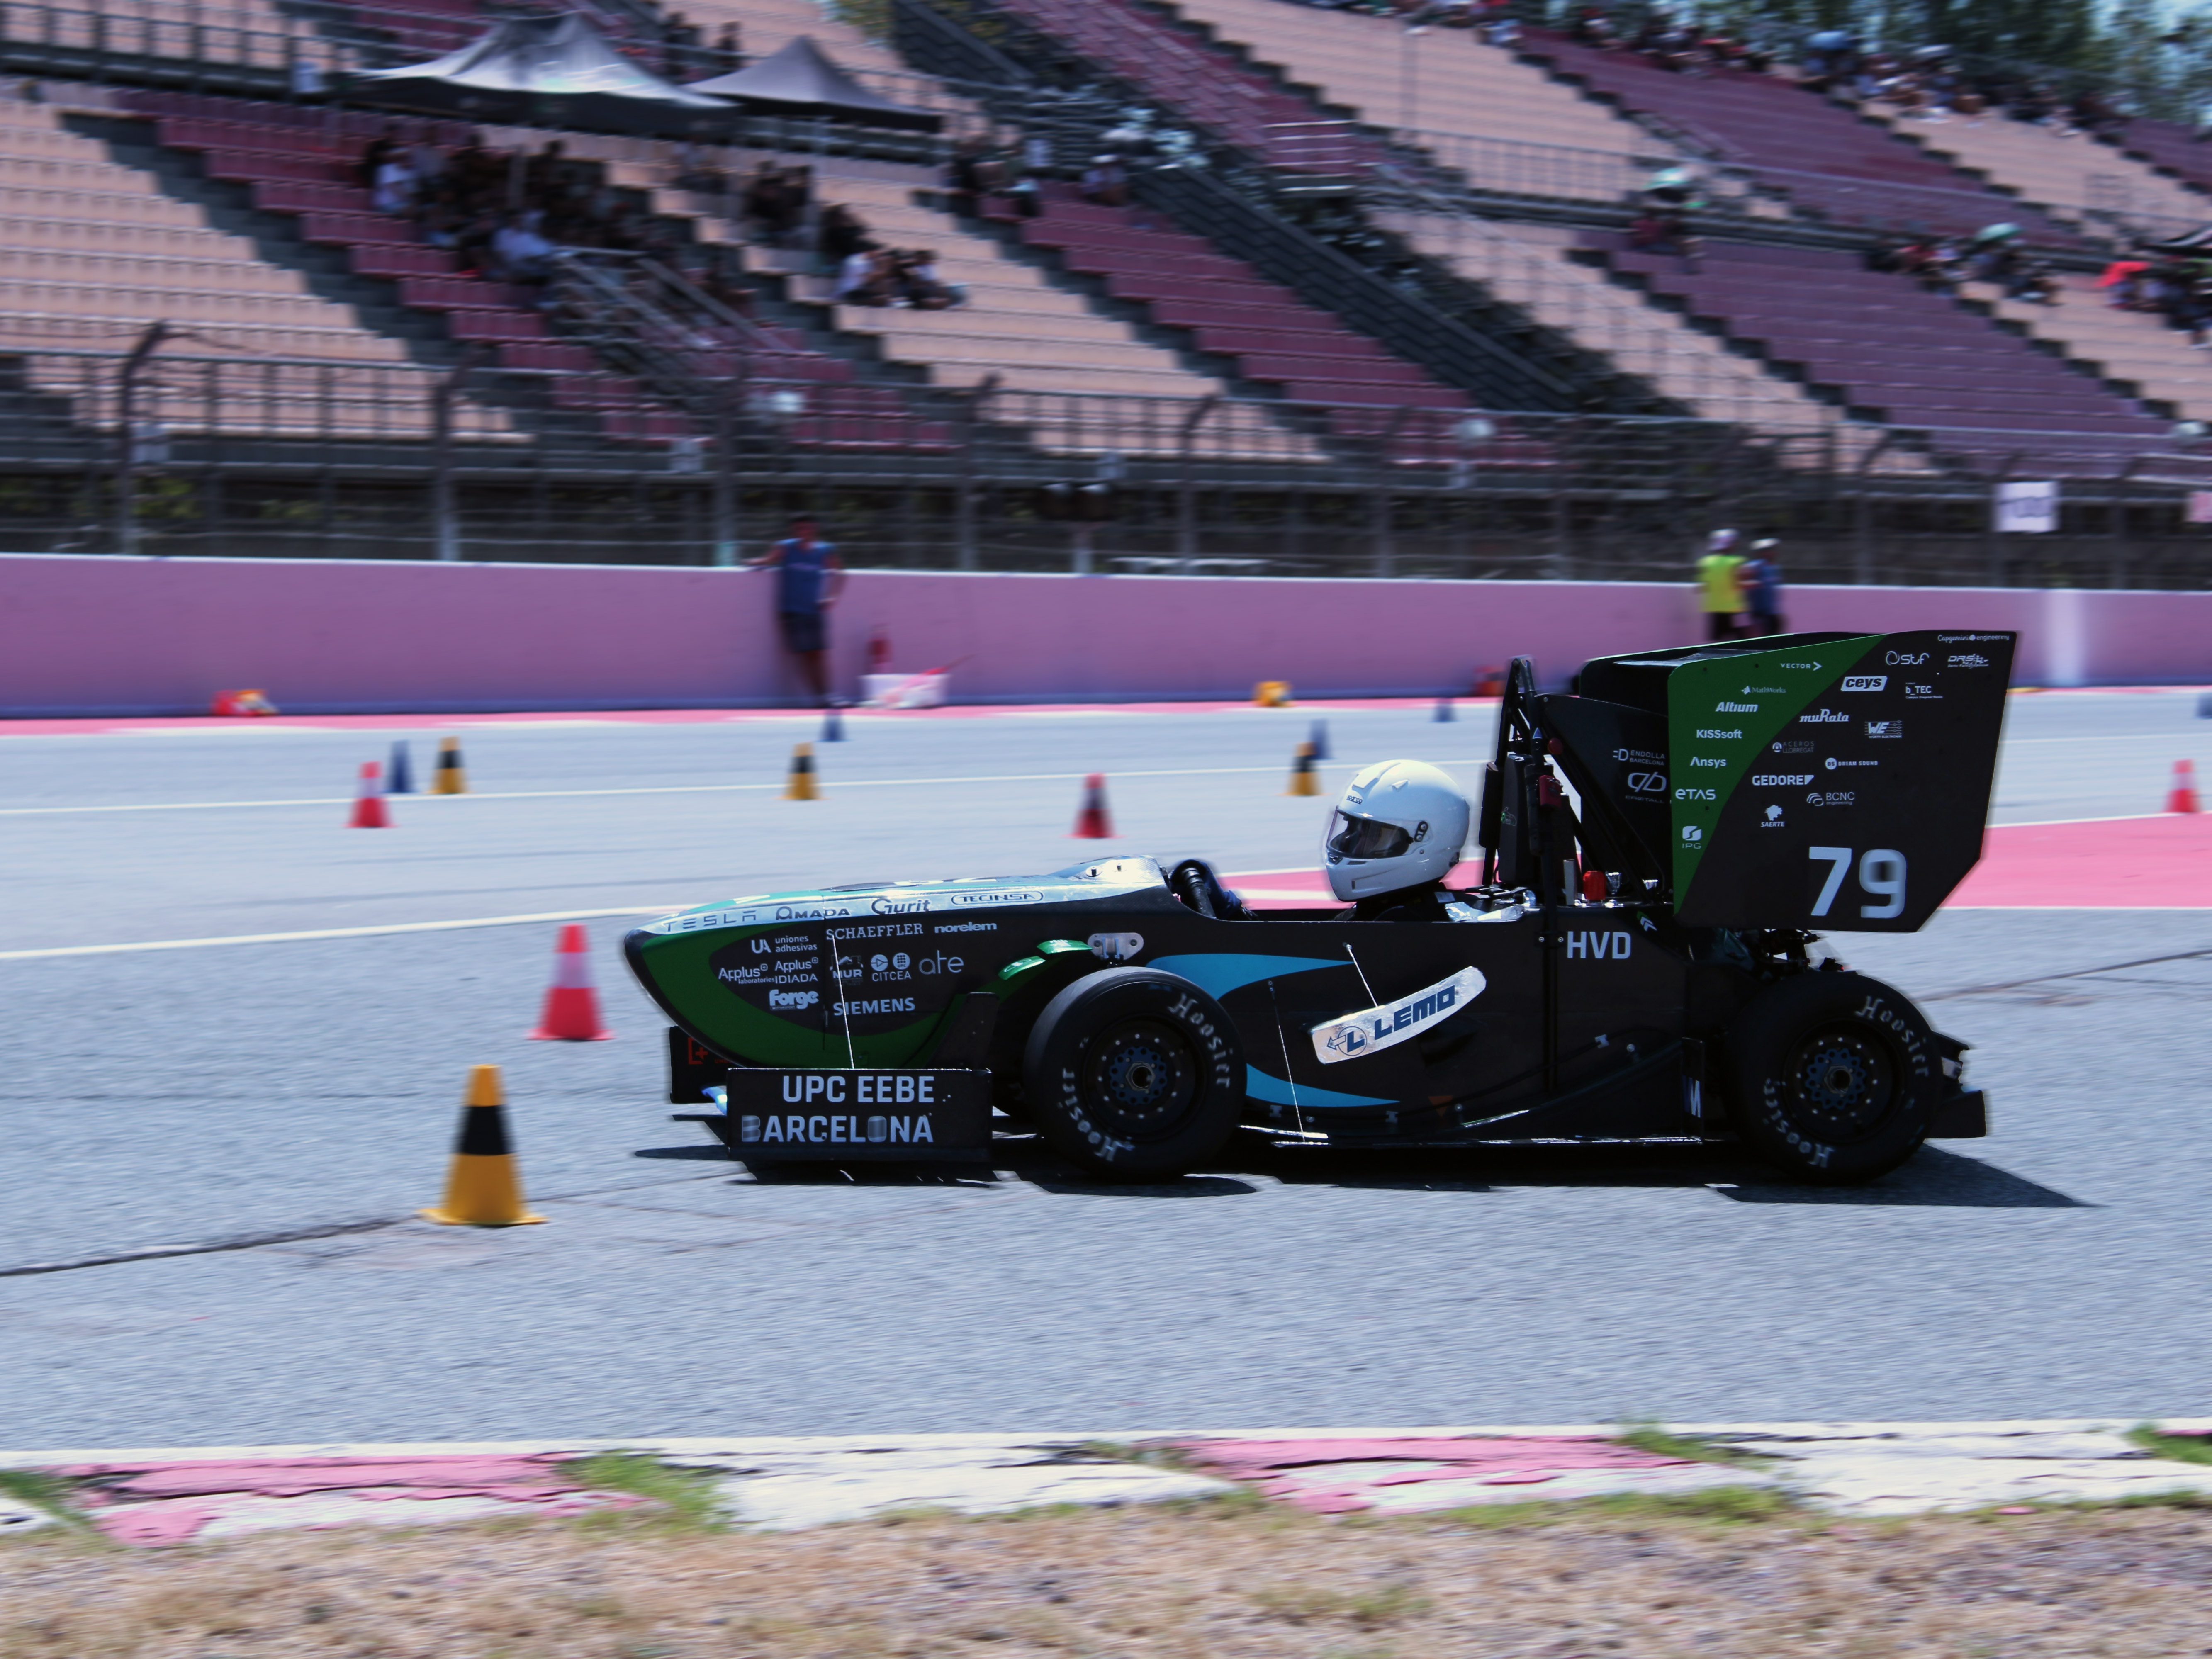
\includegraphics[width=0.7\linewidth]{fig/IMG_1834}
	\caption{ETR-08, el monoplaza con el que e-Tech Racing participó en las competiciones del verano de 2023.}
\end{figure}

Tras cinco años de evolución de la misma plataforma, el equipo se encuentra diseñando y construyendo un nuevo concepto en el momento en que se redacta este trabajo. El cambio principal son los motores eléctricos, cuyo nuevo diseño permitirá integrarlos en las propias ruedas del monoplaza debido a su compacidad, liberando así espacio del chasis. Se usarán dos motores, uno para cada rueda trasera, aunque el plan a largo plazo es implementar otros dos motores en las ruedas delanteras. Para controlarlos, se utilizarán dos inversores Bamocar D3 700-400 de la empresa alemana Unitek. Estos inversores están sobredimensionados en potencia y ocupan un espacio considerable dentro del chasis. Además, existen limitaciones en los parámetros modificables, lo que impide programar un control óptimo para el motor.

Para que el inversor sea fácilmente integrable con los futuros monoplazas del equipo, necesita contar con algunos componentes usados actualmente por el equipo. Por ejemplo, se usará el mismo microcontrolador que para el resto de ECUs \cite{Costa2024}, los mismos conectores de potencia y comunicación, y PCBs de estilos similares al resto de circuitos del monoplaza, con tal de que los fabricantes que colaboran con el equipo puedan fabricar todos los circuitos impresos del inversor. Esto permitirá una integración fluida del inversor como una ECU más del monoplaza, con el añadido de la electrónica de potencia personalizada.